\documentclass[a4j]{jarticle}
    \usepackage[dvipdfmx]{graphicx}
    \usepackage[ top=25truemm,bottom=25truemm,left=25truemm,right=25truemm]
    {geometry}
    \usepackage{ascmac}
    \usepackage{array}
    \usepackage{here}
    \usepackage{url}
    \usepackage{listings, jlisting}
    \renewcommand{\lstlistingname}{リスト}
\lstset{language=c,
  basicstyle=\ttfamily\scriptsize,
  commentstyle=\textit,
  classoffset=1,
  keywordstyle=\bfseries,
  frame=tRBl,
  framesep=5pt,
  showstringspaces=false,
  numbers=left,
  stepnumber=1,
  numberstyle=\tiny,
  tabsize=4
}
\makeatletter
\def\@thesis{matplotlibの日本語対応}
\def\id#1{\def\@id{#1}}
\def\department#1{\def\@department{#1}}

\def\@maketitle{
\begin{center}
{\huge \@thesis \par} %修士論文と記載される部分
\vspace{10mm}
{\LARGE\bf \@title \par}% 論文のタイトル部分
\vspace{10mm}
{\Large \@date\par}	% 提出年月日部分
\vspace{20mm}
{\Large \@department \par}	% 所属部分
{\Large \@id \par}	% 学籍番号部分
\vspace{10mm}
{\Large \@author}% 氏名 
\end{center}
\par\vskip 1.5em
}

\title{version1.0}
\date{2020年11月10日}
\department{}
\id{}
\author{金澤雄大}

    \begin{document}
    \maketitle
    \thispagestyle{empty}
    \clearpage
    \addtocounter{page}{-1}

    \section{Overview}
    matplotlibはデフォルトの設定では日本語を扱うことができません.
    ここでは,matplotlibの日本語対応を行う方法を解説します.想定環境は表\ref{env}です.
    \begin{table}[H]
      \caption{想定環境}
    \label{env}
    \begin{center}
        \begin{tabular}{c|l}\hline
          OS & Microsoft Windows 10 Home 64bit \\
          統合開発環境 & ANACONDA3-2020.07-Windows-x64-v8.0.4.30 \\
          Python & version3.8.5 \\
          pip & version20.2.4 \\
          matplotlib & 3.3.2 \\ \hline
        \end{tabular}
    \end{center}
    \end{table}


    日本語対応は次に示す4つのステップで行います.
    \begin{enumerate}
      \item フォントのダウンロード.
      \item matplotlibrcの修正.
      \item キャッシュの削除.
      \item 日本語対応できているか確認.
      \end{enumerate}


      \section{フォントのダウンロード}
      まず,フォントのダウンロードを行います.ここでは「Noto Sans CJK JP」というフォントでmatplotlibの日本語対応
      をします.手順は次の通りです.
      \begin{enumerate}
        \item ダウンロードページ\url{https://www.google.com/get/noto/}にアクセスします.図\ref{dlpage1}に示すページがでます.
        \item 検索窓に「JP」と入れると,図\ref{dlpage2}のように「Noto Sans CJK JP」フォントが出てきます.これをクリックすると「DOWNLOAD」が表示されるので,クリックしてダウンロードします.
        \item ダウンロードしたzipファイルを解凍すると,図\ref{dled}のようにREADME,ライセンスファイル,フォントファイルの3つがあることがわかります.
        \item Windowsのフォント設定を開きます.図\ref{fontsetteing}はフォント設定の画面です.
        \item 「ドラッグアンドドロップしてインストールします」というところに,解凍したフォルダの中の「.otf」という拡張子のファイルをすべてドラッグアンドドロップします.これでフォントのダウンロードは完了です.
        \end{enumerate}

        \begin{figure}[H]
          \centering
          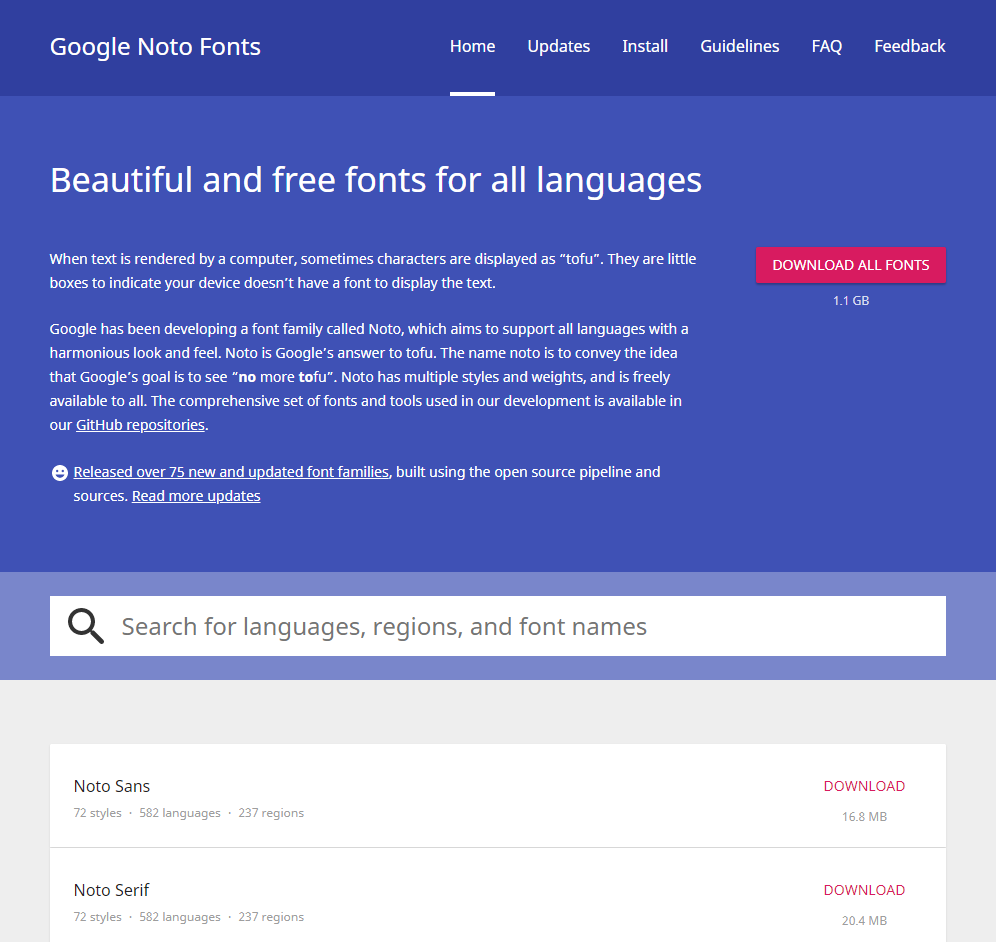
\includegraphics[scale=0.3]{downloadpage.png}
          \caption{Google Noto Fontsのダウンロードページ}
           \label{dlpage1}
          \end{figure}

          \begin{figure}[H]
            \centering
            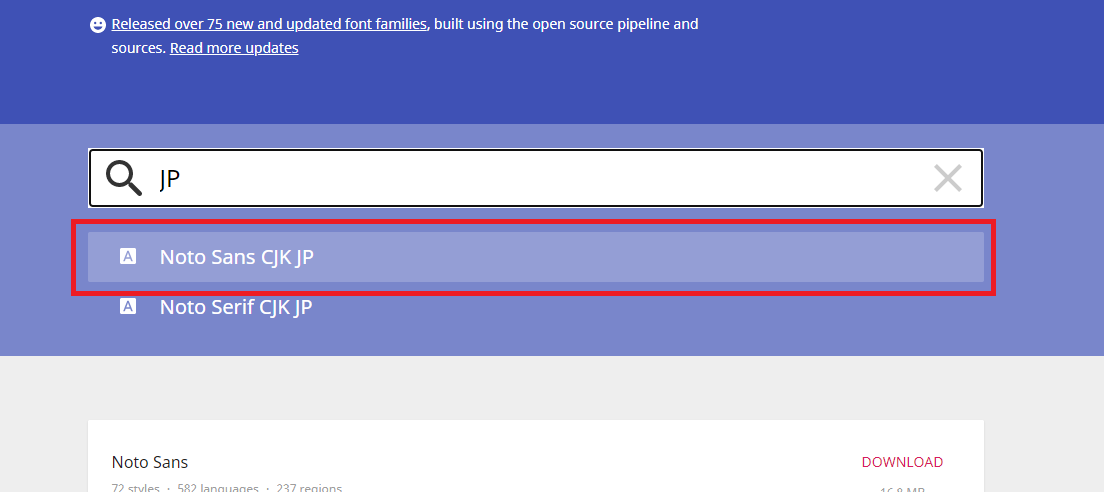
\includegraphics[scale=0.4]{fontdl.png}
            \caption{フォントのダウンロード}
             \label{dlpage2}
            \end{figure}

            \begin{figure}[H]
              \centering
              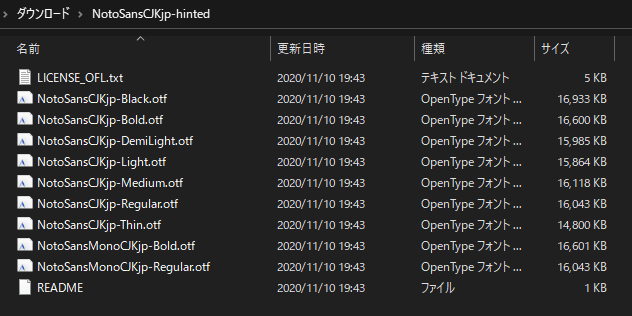
\includegraphics[scale=0.7]{dled.png}
              \caption{解凍したフォントファイル}
               \label{dled}
              \end{figure}

              \begin{figure}[H]
                \centering
                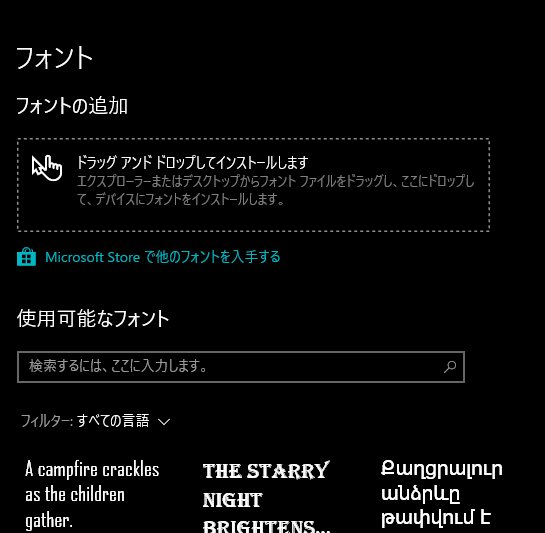
\includegraphics[scale=0.5]{fontsetting.png}
                \caption{Windowsのフォント設定画面}
                 \label{fontsetteing}
                \end{figure}
    
    \section{matplotlibrcの修正}
    matplotlibの設定ファイルを修正します.matplotlibrcの修正は次の手順で行います.
    \begin{enumerate}
      \item pythonでリスト\ref{where_rc}のプログラムを実行します.リスト\ref{where_rc}のpythonのソースコードはmatplotlibの設定ファイルである
      matplotlibrcのpathを取得するコードです.リスト\ref{where_rc}のソースを実行して表示されるpathにエクスプローラーなどを用いて潜ってください.そこにmatplotlibrcというファイルがあります.
      \item matplotlibrcの修正を行う前にこれをコピーして「User/.matplotlib」にコピーしてください.matplotlibrcをそのまま編集してもよいのですが,
      設定ファイルの読み込み優先順位が「.matplotlib」のほうが高いです.
      \item matplotlibrcの256行目付近をリスト\ref{rc_edit}のように編集します.フォント名の羅列があるので,先頭に「Noto Sans CJK JP」を追加します.
      注意点としてコメントアウト「#」を外すことを忘れないようにしてください.これでmatplotlibrcの修正は完了です.
      \end{enumerate}

      \begin{lstlisting}[basicstyle=\ttfamily\footnotesize, frame=single,label=where_rc,caption=matplotlibrcのpathを取得するコード]
import matplotlib as mpl
print(mpl.matplotlib_fname())
              \end{lstlisting}

      \begin{lstlisting}[basicstyle=\ttfamily\footnotesize, frame=single,label=rc_edit,caption=matplotlibrcの編集]
font.serif:      Noto Sans CJK JP, Bitstream Vera Serif, Computer Modern Roman, ...
font.sans-serif: Noto Sans CJK JP, Bitstream Vera Sans, Computer Modern Sans Serif,...
              \end{lstlisting}

\section{キャッシュの削除}
matplotlibのフォントのキャッシュを消去します.「User/.matplotlib」にある「fontlist-v330.json」というファイルを削除してください.
さらに,リスト\ref{rm_cash}のpythonのコードを実行してください.これらによってmatplotlibのフォントのキャッシュが削除されます.

\begin{lstlisting}[basicstyle=\ttfamily\footnotesize, frame=single,label=rm_cash,caption=キャッシュを削除するコード]
import matplotlib as mpl
mpl.font_manager._rebuild()
\end{lstlisting}

\section{日本語対応ができているか確認.}
日本語対応ができているか確認します.リスト\ref{test_jp}のpythonのコードを実行してください.図\ref{result}に示すように,ラベルに「日本語テスト」が
表示されれば成功です.
\begin{lstlisting}[basicstyle=\ttfamily\footnotesize, frame=single,label=test_jp,caption=日本語対応の確認のためのコード]
import matplotlib.pyplot as plt
x=[1,2,3]

plt.plot(x,x,label="日本語テスト")
plt.legend()
\end{lstlisting}

          \begin{figure}[H]
            \centering
            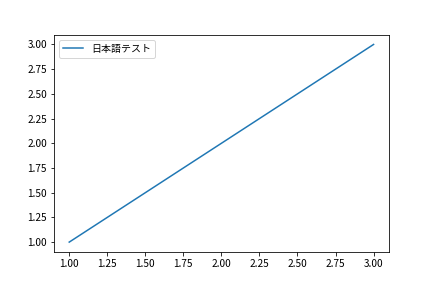
\includegraphics[scale=0.7]{result.png}
            \caption{日本語対応に成功した場合の実行結果}
             \label{result}
            \end{figure}
\end{document}

